\section{Accionaments}

Una vàlvula no canvia de posició sola: algú o alguna cosa l'ha d'\textbf{accionar}. Pot ser una persona amb un botó, un cilindre que arriba al final del recorregut, un senyal d'aire o un senyal elèctric.

\begin{idea}
L'\textbf{accionament} és el mecanisme que fa possible el canvi de posició d'una vàlvula (de repòs a treball i a l'inrevés). Es dibuixa \textbf{a un costat de la vàlvula} i el \textbf{retorn} a l'altre. Pot ser:
\begin{itemize}
 \item \textbf{Muscular} (el fa una persona): manual, polsador, palanca, pedal.
 \item \textbf{Mecànic}: rodet (final de cursa) i molla (retorn).
 \item \textbf{Pneumàtic}: un senyal d'aire a pressió (pilotatge).
 \item \textbf{Elèctric}: una tensió que activa un solenoide (electrovàlvula).
\end{itemize}
\end{idea}

\subsection*{Els accionaments més habituals}

\begin{center}
\renewcommand{\arraystretch}{1.1}
\begin{tabular}{@{}c l c l@{}}
\toprule
\textbf{Símbol} & \textbf{Accionament} & \textbf{Símbol} & \textbf{Accionament}\\
\midrule
\simb{\pnvalve{x}{0}{0}{32nc}{man}{spring}}\hspace{1.2cm} & \textbf{Manual general} &
\simb{\pnvalve{x}{0}{0}{32nc}{pol}{spring}}\hspace{1.2cm} & \textbf{Polsador}\\[2.1em]
\simb{\pnvalve{x}{0}{0}{32nc}{lever}{spring}}\hspace{1.2cm} & \textbf{Palanca} &
\simb{\pnvalve{x}{0}{0}{32nc}{pedal}{spring}}\hspace{1.2cm} & \textbf{Pedal}\\[2.1em]
\simb{\pnvalve{x}{0}{0}{32nc}{roll}{spring}}\hspace{1.2cm} & \textbf{Rodet} (final de cursa) &
\simb{\pnvalve{x}{0}{0}{32nc}{pilot}{spring}}\hspace{1.2cm} & \textbf{Pneumàtic} (pilotatge)\\[2.1em]
\simb{\pnvalve{x}{0}{0}{32nc}{elec}{spring}}\hspace{1.2cm} & \textbf{Elèctric} (electrovàlvula) &
\simb{\pnvalve{x}{0}{0}{32nc}{pol}{pilot}}\hspace{1.2cm} & Polsador i \textbf{pneumàtic}\\
\bottomrule
\end{tabular}
\end{center}

La \textbf{molla} (el símbol en zig-zag) és l'element de \textbf{retorn}: quan deixem d'accionar la vàlvula, la molla la fa tornar a la posició de repòs.

\subsection*{Monoestable i biestable}

\begin{center}
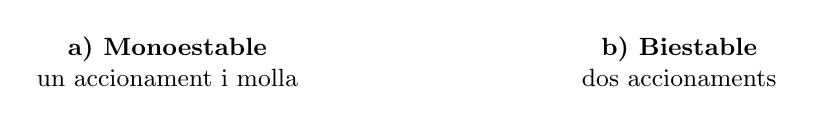
\begin{tikzpicture}[x=1cm,y=1cm]
 \pnvalve{a}{0}{0}{52}{pilot}{spring}
 \node[font=\small,align=center] at (1.4,-1.4) {\textbf{a) Monoestable}\\un accionament i molla};
 \pnvalve{b}{6.5}{0}{52}{pilot}{pilot}
 \node[font=\small,align=center] at (7.9,-1.4) {\textbf{b) Biestable}\\dos accionaments};
\end{tikzpicture}
\end{center}

\begin{idea}
\begin{itemize}
 \item Una vàlvula \textbf{monoestable} té \textbf{una sola posició estable}: la de repòs. Quan deixem d'accionar-la, la \textbf{molla} la fa tornar-hi.
 \item Una vàlvula \textbf{biestable} té \textbf{dues posicions estables}. Es queda en la posició on l'ha deixada l'últim senyal: té \textbf{memòria}. Per canviar de posició, cal un senyal a l'altre accionament.
\end{itemize}
\end{idea}

\begin{exemple}{monoestable o biestable?}
Quan premem un botó d'un timbre sona, i quan el deixem anar para. Això és un comportament \textbf{monoestable}: torna sol a repòs. En canvi, un interruptor de la llum es queda on el deixes: és \textbf{biestable}.
\end{exemple}

\subsection*{El final de cursa (rodet)}

Una vàlvula amb \textbf{rodet} es col·loca de manera que la tija d'un cilindre la toqui quan arriba al final del recorregut. Així la vàlvula \textbf{detecta} que el cilindre ja ha acabat el moviment i pot donar la ordre següent, sense que ningú hagi de prémer res. És el que fa possible que un circuit funcioni \textbf{automàticament}.

\begin{atencio}
No confonguis el \textbf{rodet} (el toca un objecte que es mou) amb el \textbf{polsador} (el prem una persona). Els símbols són diferents!
\end{atencio}

\begin{guiada}{el nom complet d'una vàlvula}
Per dir com és una vàlvula, es diu el tipus (vies/posicions) i els seus accionaments. Per exemple:
\begin{center}\simb{\pnvalve{x}{0}{0}{32nc}{roll}{spring}}\end{center}
\pas{1}{Vies/posicions:}{\vspace{0.6cm}}
\pas{2}{Accionament:}{\vspace{0.6cm}}
\pas{3}{Retorn:}{\vspace{0.6cm}}
\resposta{0pt}{Vàlvula 3/2, accionada per rodet, amb retorn per molla (normalment tancada).}
\end{guiada}

\subsection*{Exercicis}

\begin{exercici}{1}
Escriu el nom de l'accionament de cada vàlvula:\\[0.3em]
\begin{center}
\begin{tikzpicture}[x=1cm,y=1cm]
 \pnvalve{a}{0}{0}{32nc}{pedal}{spring} \node at (1.5,-1.1) {\textbf{a)}};
 \pnvalve{b}{3.8}{0}{32nc}{roll}{spring} \node at (5.3,-1.1) {\textbf{b)}};
 \pnvalve{c}{7.6}{0}{32nc}{elec}{spring} \node at (9.1,-1.1) {\textbf{c)}};
 \pnvalve{d}{11.4}{0}{32nc}{pilot}{spring} \node at (12.9,-1.1) {\textbf{d)}};
\end{tikzpicture}
\end{center}
\resposta{0cm}{a) Pedal; b) rodet; c) elèctric (solenoide); d) pneumàtic (pilotatge).}
\end{exercici}

\begin{exercici}{1}
Quina és la utilitat principal de les vàlvules accionades per rodet?
\resposta{2cm}{Detecten quan una tija (o un objecte en moviment) arriba a una posició, com un final de cursa; permeten automatitzar el circuit.}
\end{exercici}

\begin{exercici}{2}
Observa les dues vàlvules i digues quina és monoestable i quina és biestable. Raona-ho.\\[0.3em]
\begin{center}
\begin{tikzpicture}[x=1cm,y=1cm]
 \pnvalve{a}{0}{0}{52}{pol}{spring} \node at (1.7,-1.1) {\textbf{a)}};
 \pnvalve{b}{7}{0}{52}{pilot}{pilot} \node at (8.4,-1.1) {\textbf{b)}};
\end{tikzpicture}
\end{center}
\resposta{3.2cm}{a) és monoestable: té un polsador i una molla de retorn, i en deixar anar el polsador torna a repòs. b) és biestable: té un accionament a cada costat, no té molla i es queda a la posició on l'ha deixada l'últim senyal (té memòria).}
\end{exercici}

\begin{exercici}{2}
Quin accionament triaries per a cada situació? Raona-ho.\\
a) Una porta d'autobús que s'obre quan el conductor prem un botó. \ b) Detectar que un cilindre ha arribat al final del recorregut. \ c) Una màquina que és controlada per un ordinador.
\resposta{3.6cm}{a) Polsador (acció d'una persona). b) Rodet (el toca la tija del cilindre). c) Elèctric (electrovàlvula): l'ordinador dóna un senyal elèctric.}
\end{exercici}

\begin{exercici}{3}
Descriu amb paraules aquesta vàlvula: tipus, accionament i retorn. Quan es produeix cada posició?\\
\begin{center}\simb{\pnvalve{x}{0}{0}{42}{pedal}{spring}}\end{center}
\resposta{3cm}{Vàlvula 4/2 accionada per pedal i amb retorn per molla. En repòs (molla) l'aire va de 1 a 4; quan trepitgem el pedal passa de 1 a 2. En deixar el pedal, la molla la fa tornar a repòs.}
\end{exercici}

\begin{comprova}
Una vàlvula amb accionament a cada costat i sense molla és\ldots\ \ $\square$ monoestable \quad $\square$ biestable
\resposta{0pt}{Biestable.}
\end{comprova}
